% vim:ts=4:sw=4
% Copyright (c) 2014 Casper Ti. Vector
% Public domain.

\chapter{基于PUF建模的仿真分析和设计方法}\label{chap:buildingmodel}
\section{双稳环路PUF的建模分析}\label{sec:brpufmodel}

上一章中介绍了双稳态环路 PUF(BRPUF),在本章节中我们将对 BRPUF 建模分析,指出在电路结构上影响 PUF 输出分布的几个因素。

\subsection{偶数级环路振荡器}

BRPUF 的一个单元包含了两个选择器和与非门,整体延迟比较大,而仿真发现,延迟较大的反相器构成的偶数级环路并不会迅速稳定。

\begin{figure}[htb!]
\centering
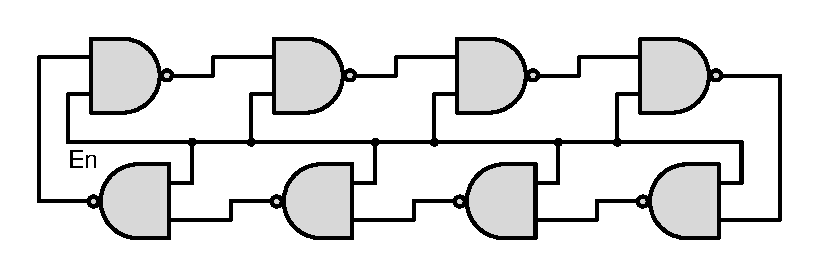
\includegraphics[width=\linewidth]{bistable-ring}
\caption{偶数级环路}
\label{fig:bistable-ring}
\end{figure}

\begin{figure}[htb!]
\centering
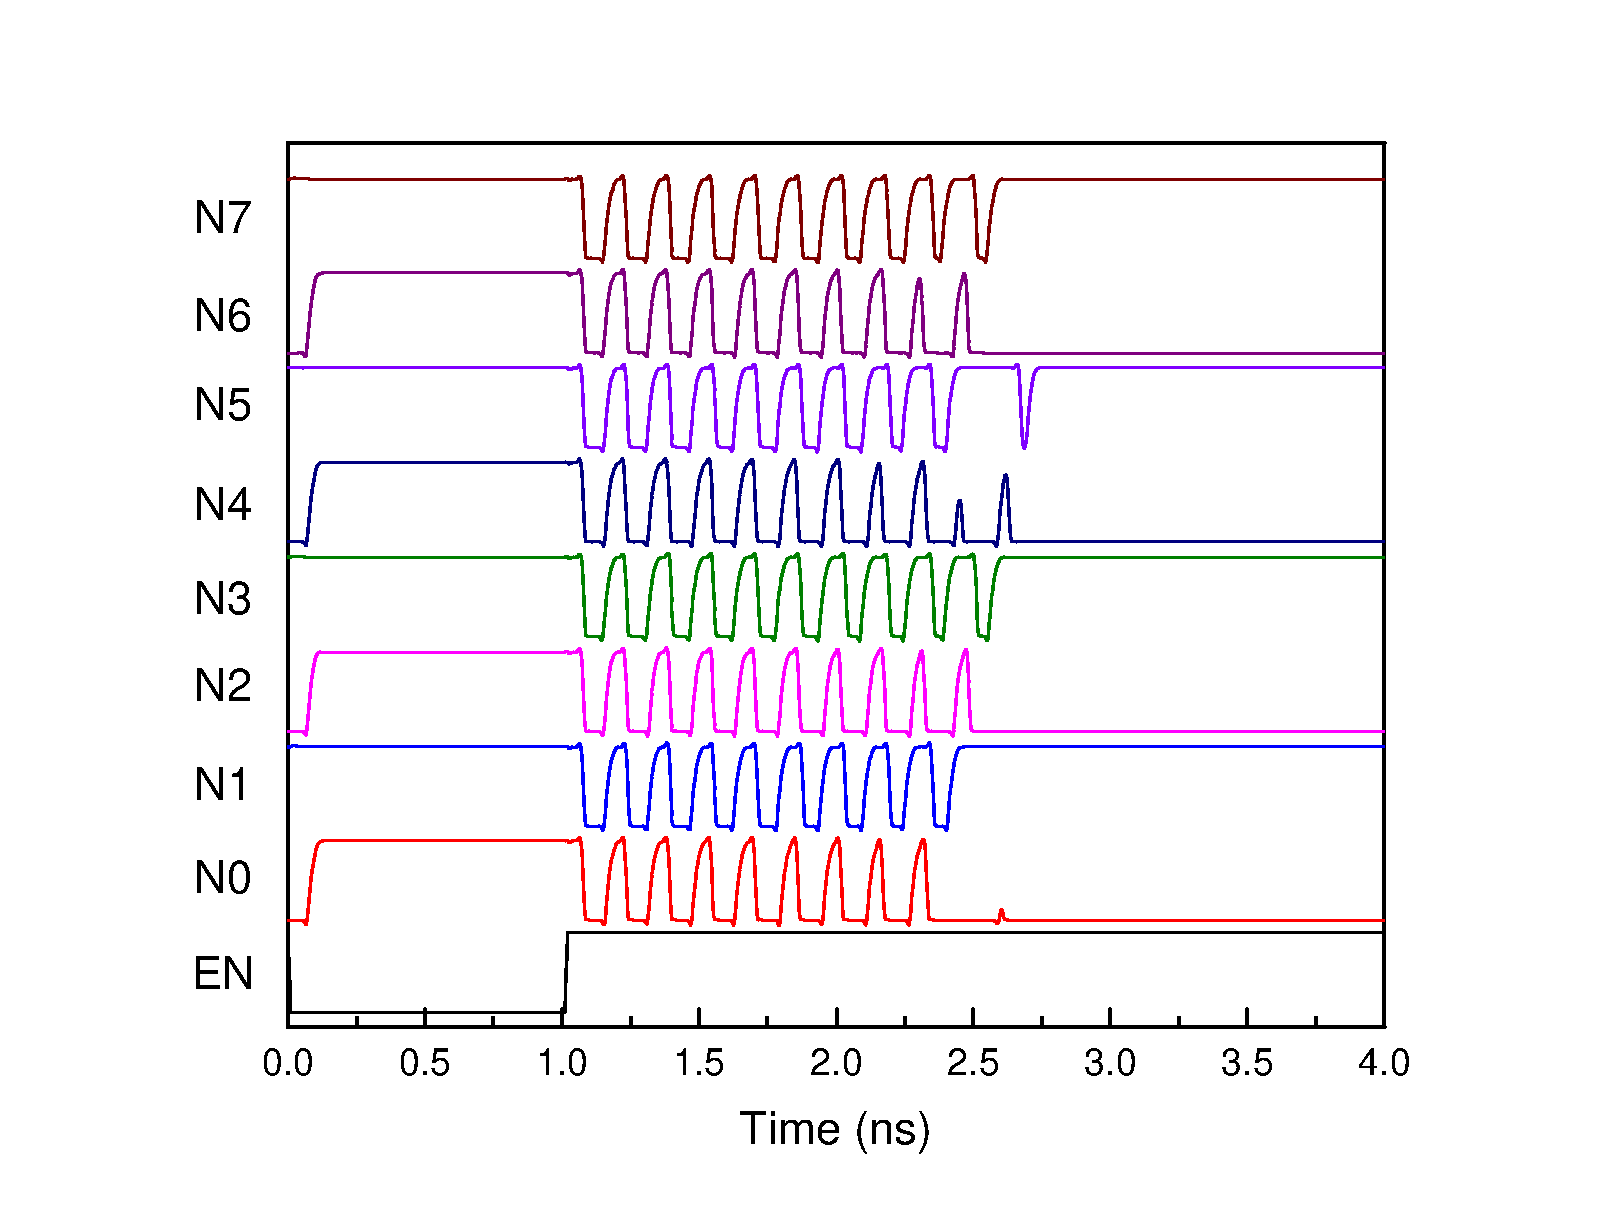
\includegraphics[width=\linewidth]{br_waveform}
\caption{偶数级环路仿真波形图}
\label{fig:brwaveform}
\end{figure}

如图\ref{fig:bistable-ring}所示,环路由$ N=8 $个与非门组成,当EN信号为低时,所有节点处于充电状态,当EN信号上跳时,电路开始进入``震荡状态''(如图\ref{fig:brwaveform}所示)。由于每个与非门的延迟时间远大于信号的上升时间和下降时间,故建立如下的模型:

\textbf{定义1:}第i个与非门的0-1上升延迟为$ tr_i $,1-0下降延迟为$ tf_i $。

当一个占空比为W的方波通过与非门i后,输出方波占空比变为:
\begin{equation}
W_{i+1}=W_i+\frac{tf_i-tr_i}{T}
\end{equation}
其中T为方波周期。当EN信号上跳后,初始占空比为$ W_0 $的方波激励输入与非门i,输出占空比为$ W_1 $,动态的考虑这个方波,当它经过N个与非门驱动后环回初始的节点,其占空比变为:
\begin{equation}
W_N=W_0+\sum\limits_{i=0}^{N}\frac{(-1)^i(tf_i-tr_i)}{T}=W_0+\Delta W
\end{equation}
当 $ \Delta W>0 $ ,则占空比趋向于1,意味着i与非门的输出节点最终收敛到逻辑``1'',反之则说明i与非门输出节点收敛到逻辑``0''。当 $ \Delta W=0 $ 时,占空比不发生变化,只要在一个环回周期内占空比不会变为1或0,那么电路将``理想''得 振荡下去,因此称其为偶数级环振。

\textbf{定义2:}环路中信号周期定义为所有逻辑门延迟之和。节点k的一次震荡(1次下跳和1次上跳)称为一个子周期。

\textbf{推论1}:N级环路(如不特别说明,此后环路中N为偶数)如不收敛,一个信号周期内节点k经历N/2个子周期;

\textbf{推论2}:偶数级环振振荡次数 $ M \propto \frac{W_0}{\Delta W}\cdot\frac{N}{2} $ ,故与非门上升下降延迟之差越小,延迟差总和越小,振荡次数越大。

振荡次数会影响 BRPUF 的求值时间,而且越久的振荡越容易收到噪声扰动使得电路不能在求值周期内收敛或者随机收敛。

\subsection{BRPUF模型}\label{subsec:brpufmodel}
接下来考虑图\ref{fig: brpuf}中的 BRPUF 电路,记激励 $ c_i\in{-1,1} $,一个单元内两个与非门的上升延迟和下降延迟分别为$ p,q,r,s $,取下标系数为0的与非门输出信号作为响应R。根据上一节分析知,响应R有:
\begin{equation}\label{eq:brmodel}
R=sgn(\sum\limits_{i=0}^{N}(-1)^i(\frac{1+c_i}{2}(p-q)+\frac{1-c_i}{2}(r-s)))=sgn(\sum(\alpha_i c_i+\beta_i))
\end{equation}
其中$ \alpha_i=(-1)^i\frac{p_i-q_i-r_i+s_i}{2} $, $ \beta_i=(-1)^i\frac{p_i-q_i+r_i-s_i}{2} $,类比\ref{subsec:apufmodel}节中的工作,可以将R写成
\begin{equation}
R=sgn(p'd)
\end{equation}
这是一个线性表达式,所以对于N级 BRPUF,则在N维空间中存在超平面可以将 CRP 区分开。在\ref{sec:modelverify}节中我们将演示用 SVM 拟合 FPGA 上的 BRPUF 参数向量d。

\subsection{BRPUF输出统计特性}\label{subsec:brpuf_stat}
在\ref{subsec:metrics}小节中介绍了 PUF 的几个评价指标,其中随机性、独特性和可靠性是 PUF 的统计特性,为了方便起见,定义工艺波动呈正态分布,故由工艺波动导致的单元延迟时间$ p,q,r,s $也近似呈正态分布。

\textbf{假设1:} BRPUF 单元延迟时间服从正态分布,即$ p,q,r,s \sim N(\mu,\sigma) $。

由 BRPUF 的模型式\ref{eq:brmodel}可知,$ R=sgn(\delta),\delta=\sum(\alpha c+\beta)=A'C+B $,则在随机性统计中,样本容量最大为$ 2^N $(N为激励位数),所以
\begin{equation}\label{eq:mean_delta}
\mu(\delta)=\frac{\sum A'C}{2^N}+B
\end{equation}
从0取到$ 2^N-1 $过程中,任意一位$ c_i $总是 一半为1, 一半为-1,所以式\ref{eq:mean_delta}前者之和为0,故有$ \mu(\delta)=B $。

同理可得
\begin{equation}
\sigma(\delta)=\frac{1}{2^{N/2}}\sqrt{\sum(A'C)^2}=\sqrt{\sum\alpha_i^2}
\end{equation}
\textbf{假设2:}PUF 芯片内各晶体管工艺波动分布类似,可令$ p,q,r,s $服从正态分布的均值和标准差相等,即对$ \forall i,\mu(p_i )=\mu(q_i )=\mu(r_i )=\mu(s_i )=\mu_i,\sigma(p_i )=\sigma(q_i )=\sigma(r_i )=\sigma(s_i )=\sigma_i $。

由B的表达式可得:
\begin{equation}
B\sim N(\mu_B,\sigma_B)
\end{equation}
\begin{equation}
\mu_B=\sum\mu(\beta_i)=0
\end{equation}
\begin{equation}
\sigma_B=\sqrt{\sum\sigma^2(\beta_i)},\sigma(\beta_i)=\dfrac{\sqrt{\sigma^2(p_i)+\sigma^2(q_i)+\sigma^2(r_i)+\sigma^2(s_i)}}{2}=\sigma_i
\end{equation}
故B的分布均值为0,标准差是单个单元延迟标准差的$ \sqrt{N} $倍。

对于单个 PUF 芯片的随机性统计,若B严格为0,则随机性严格地为50\%。若要求随机性的下限不得低于$ Rn_L $,上线不得高过$ Rn_H $,根据统计学知识,$ Rn=\frac{1}{2}erfc(x) $,其中 erfc 是余误差函数,$ x=-\frac{B}{\sqrt{2}\sigma(\delta)} $。故设一个 BRPUF 芯片随机性Rn满足条件的概率为P:
\begin{equation}
P=\int\limits_{Rn_L}^{Rn_H}\dfrac{Rn\cdot dx}{\int\limits_{-\infty}^{+\infty}Rn\cdot dx}
\end{equation}
根据 Matlab 的模拟,$ \mu(\delta) $的分布的标准差与$ \sigma(\delta) $的分布标准差比值$ \frac{\sigma(\mu(\delta))}{\sigma(\sigma(\delta))} $ 越大, Rn 分布的尖峰越高,比值为1时 Rn 呈随机分布,比值小于1, Rn 呈谷型分布。由假设2, BRPUF 的比值接近于1,故P近似于$ Rn_H-Rn_L $。

根据 PUF 独特性的定义,Rn接近50\%的概率越大,独特性越接近50\%;反之,说明多个 PUF 中大量个体输出分布偏差很大,个体之间汉明距离跟趋向于0和N两个极限值。

而可靠性主要考虑$ p,q,r,s $随环境变化对$ sgn(\delta) $的影响。

综上我们得到: BRPUF 的随机性和独特性较低。


\section{基于统计分析的PUF设计方法}
可以将\ref{sec:brpufmodel}节的分析推广开。第一代PUF\footnote{\parencite{rostami2014quo}中对PUF的总结,区别于Digital PUF}由3部分组成:物理信息转换模块,仲裁模块和输出模块。

若输出数字电路信号,则物理信息转换模块一定能写成 $ p’d $ 的形式,但 p,d 向量的维度不一定是激励的位宽,维度越大,说明转换过程越复杂;在上面的几个例子中,仲裁模块都是 sgn 函数,实际上任何二值逻辑输出都能等价为 sgn 函数;输出模块取决于整体系统设计,可以异或多个 PUF 的响应,也可以添加投票机制以提高稳定性\supercite{mathew201416}。

由\ref{sec:brpufmodel}节讨论可知, PUF 随机性Rn与 $ \frac{\sigma(\mu(\delta))}{\sigma(\sigma(\delta))} $ 相关,且比值应越大越好。

PUF 的随机性分布与独特性有关联,两个独立 PUF 元件的随机性分别为$ Rn_1,Rn_2 $,则两个 PUF 由N个随机激励产生的响应 R1,R2 的汉明距离 HD 有:
\begin{equation}
N|Rn_1-Rn_2|\leq HD\leq N\times min{Rn_1+Rn_2,2-Rn_1-Rn_2}
\end{equation}

推导HD的分布相当复杂,本文仅根据Matlab仿真得到定性结论:
\begin{itemize}
\item 只要Rn分布的均值是0.5,则HD的分布是均值0.5的高斯分布;
\item Rn的方差越小,HD的方差也越小,反之HD的方差越大;
\item Rn的方差与 $ \frac{\sigma(\mu(\delta))}{\sigma(\sigma(\delta))} $ 有关,比值越大,方差越大;
\end{itemize}

事实上上述比值的分母由工艺条件决定,在电路实际制造中往往希望工艺波动即分母越小越好,这不利于 PUF 的实现,所以 PUF 的设计应该在此基础上使转换值的均值分布方差越小。


\section{模型验证}\label{sec:modelverify}
\subsection{仿真验证}\label{subsec:simu}
仿真采用 HSPICE 和 Matlab 模拟结合的方法,因为单用 HSPICE 这类动态仿真软件难以在有限时间内模拟大量数据。根据H SPICE SMIC 40nm 的库文件,取栅长 L=40nm, PMOS 有源区宽$ W_p=200 $nm, NMOS 有源区宽$ W_n=120 $nm。提取出蒙特卡洛仿真的参数,经过10000次蒙特卡洛得到带负载的反相器和与非门延迟分布(如图\ref{fig:inv-delay},图 \ref{fig:nand-delay}所示)。

\begin{figure}[htb!]
\centering
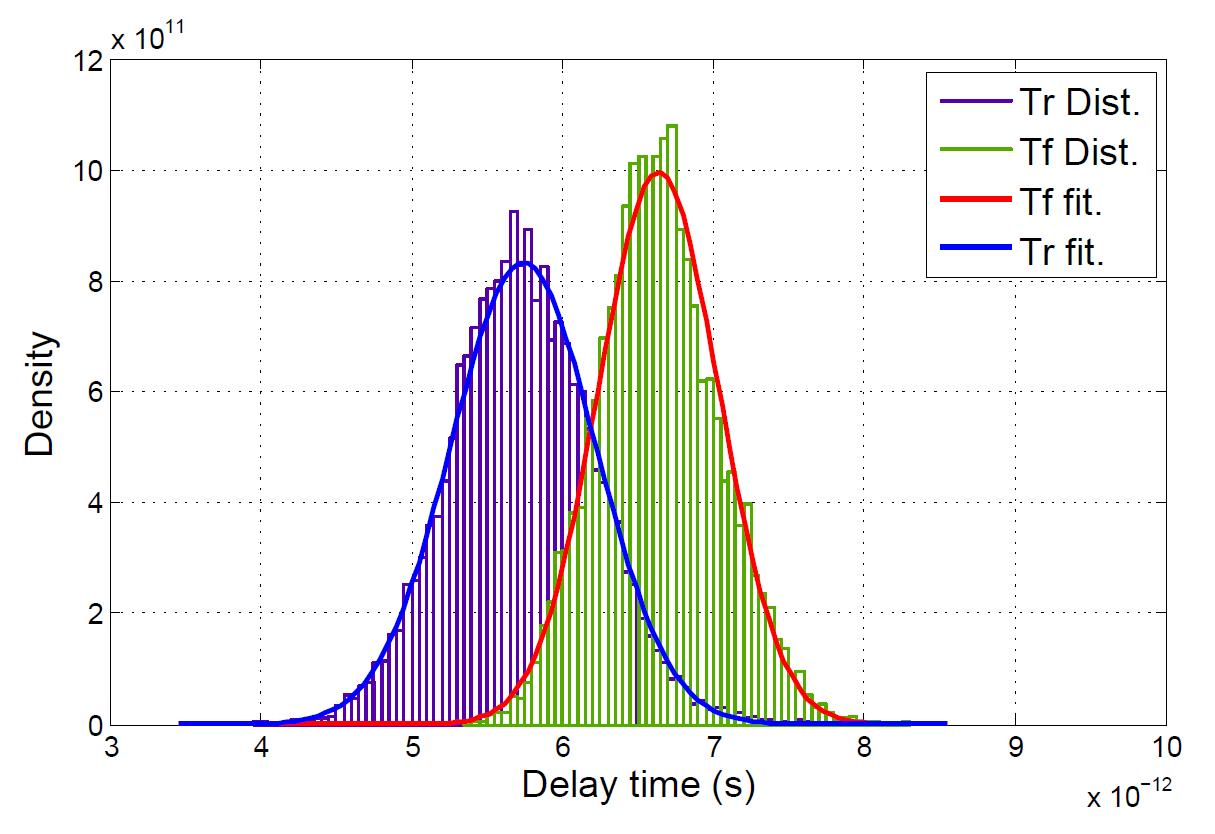
\includegraphics[width=.8\linewidth]{INV_Delay_Dist}
\caption{反相器延迟分布图}
\label{fig:inv-delay}
\end{figure}

\begin{figure}[htb!]
\centering
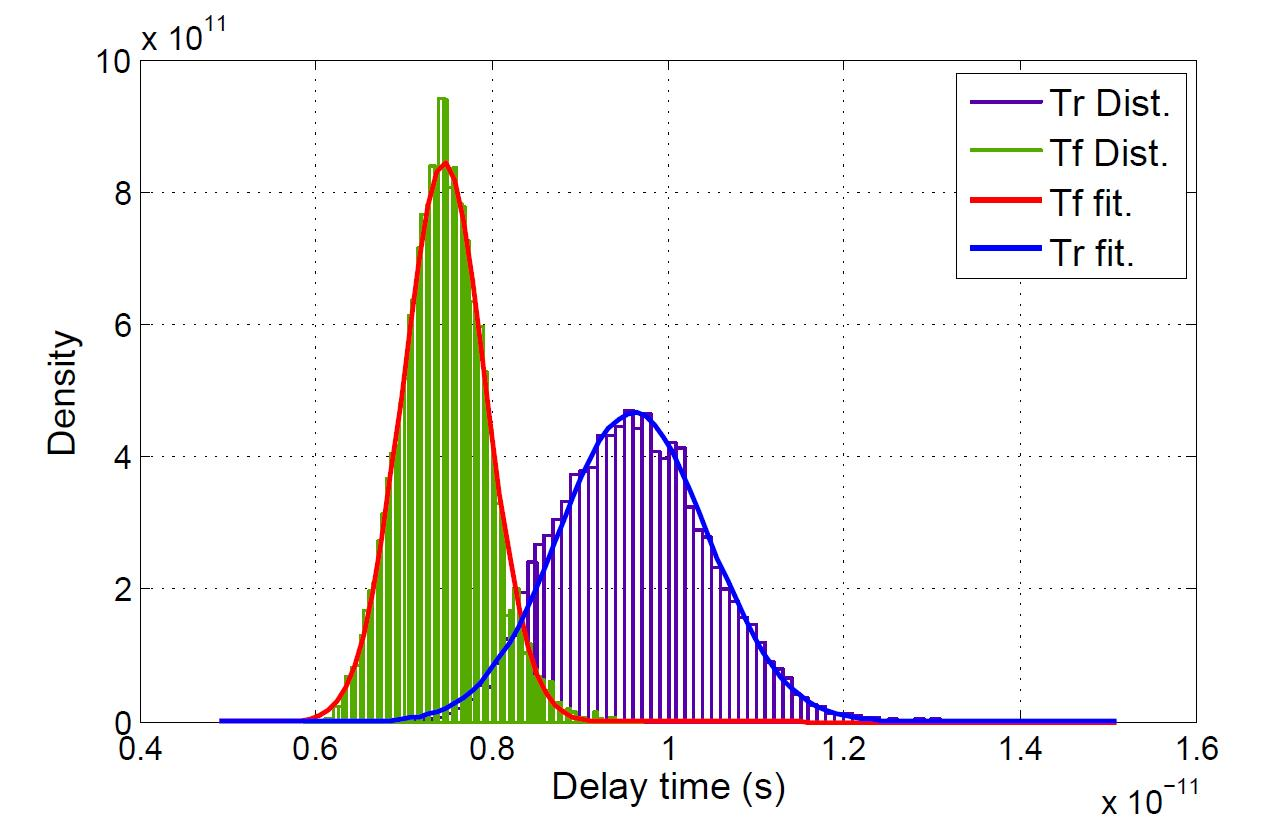
\includegraphics[width=.8\linewidth]{Nand_Delay_Dist}
\caption{与非门延迟分布图}
\label{fig:nand-delay}
\end{figure}

拟合出反相器延迟服从$ tr: N\sim(5.74\times 10^{-12},4.79\times 10^{-13}) $, $ tf: N\sim(6.64\times 10^{-12},4.00\times 10^{-13}) $,与非门延迟分布服从$ tr: N\sim(9.61\times 10^{-12},8.54\times 10^{-13}) $,$ tf: N\sim(7.46\times 10^{-12},4.72\times 10^{-13}) $,用 Matlab normrnd 函数生成一个 $ M\times 4 $ 的参数矩阵,其中4列分别代表每一级$ p,q,r,s $四个延迟参数,$ M $表示 BRPUF 的级数,这里取$ M=32 $。

将参数矩阵带入模型,按平均分布随机给定1000个32位激励值,得到1000位的响应向量。重复生成1000个参数矩阵(激励保持不变),最终得到一个$ 1000\times 1000 $的响应矩阵R。

由R的每一行求和除以$ M $可以得到一个随机性数值$ Rn_i $,任意两行之间做异或求和再除以$ M $,得到相对汉明距离$ HD_j $,HD的均值就是独特性Un,图\ref{fig:brpufrand},\ref{fig:brpufuniq}画出了 BRPUF 的 Rn 和 HD 的分布。

\begin{figure}[htb!]
\centering
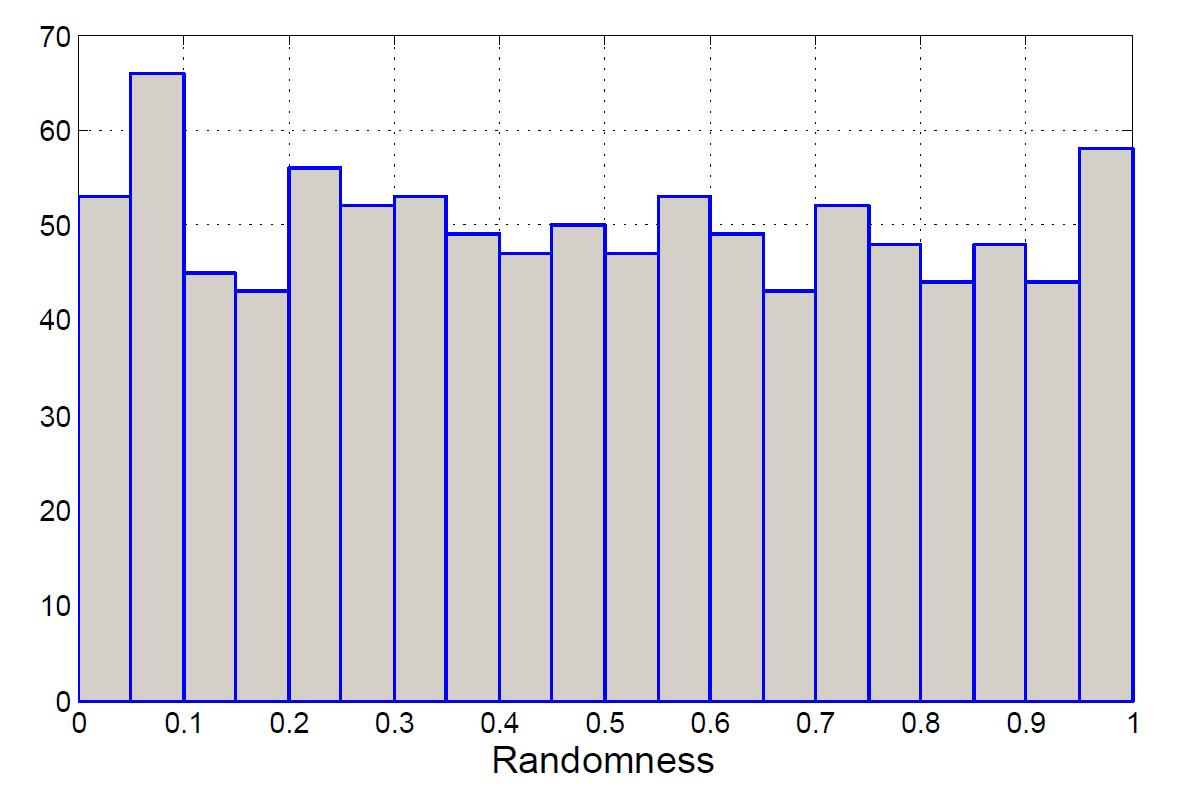
\includegraphics[width=.8\linewidth]{brpuf_rand_simulation}
\caption{BRPUF 随机性分布}
\label{fig:brpufrand}
\end{figure}

\begin{figure}[htb!]
\centering
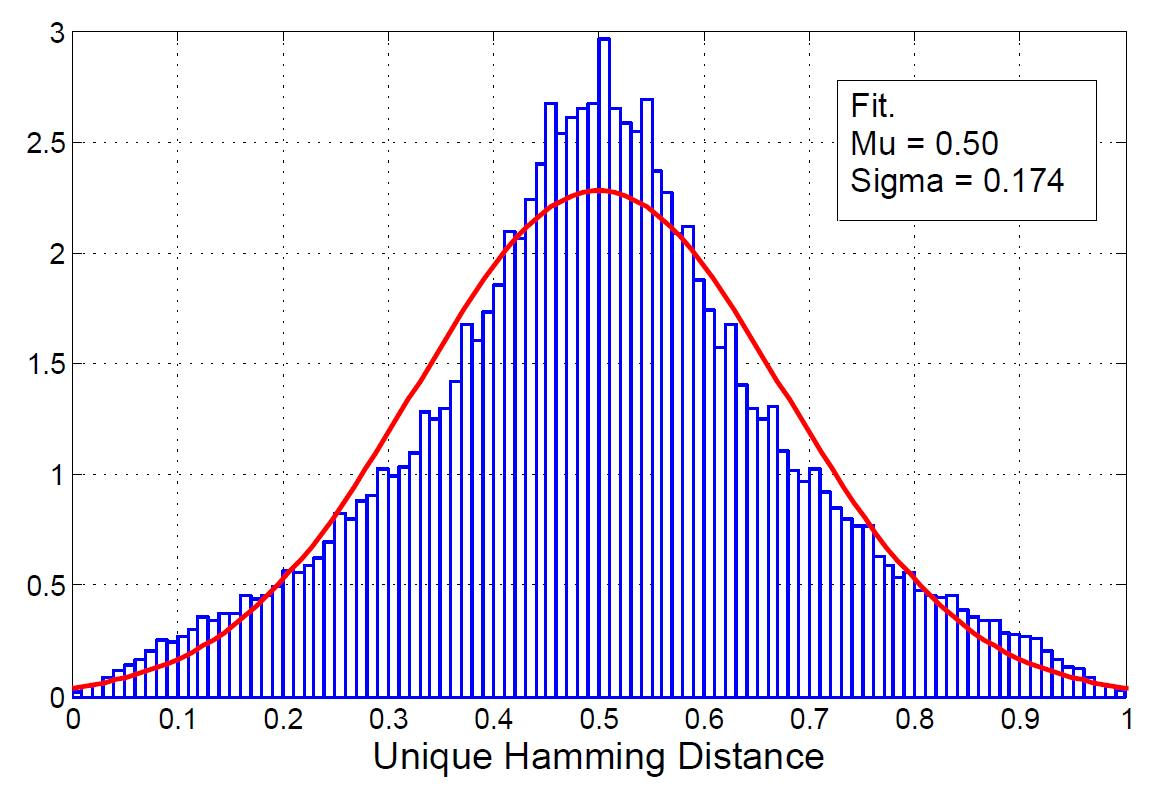
\includegraphics[width=.8\linewidth]{brpuf_uniq_simulation}
\caption{BRPUF 独特性分布}
\label{fig:brpufuniq}
\end{figure}

可以看到仿真结果和分析结论一致。 BRPUF 随机性的分布接近平均分布,独特性均值接近0.5但偏差较大,$ 3\sigma>0.5 $。

\subsection{FPGA验证}\label{subsec:fpga}
为了进一步验证理论分析结论,我们在 Altera Stratix V FPGA 芯片上实现了 BRPUF,其中一级单元用4个 LUT\footnote{Look Up Table,FPGA的基本逻辑单元} 实现,每个单元通过 Logiclock\footnote{逻辑锁定,Altera器件上固定LUT位置的工具} 固定在特定坐标的 LAB\footnote{Logic Array Blocks,由数个基本单元构成的逻辑块} 上,以保持布线平衡。读出逻辑通过 PCI-E 接口通信,在 PC 上给予激励和收集响应。并且根据 BRPUF 易振荡的特点,设定超时逻辑——以 250 MHz 时钟频率连续采样1000个输出,若连续100个保持恒定值则输出该值,否则认为没有在 $ 4\mu s $ 内收敛,输出 0xFF 表示该值无效。

我们在3块 FPGA 芯片上,每块放置30个 PUF,分别在不同的位置以模拟片间差异,一共90个 PUF,每个 PUF 收集1000个 CRP 。图\ref{fig:brpuffpga}展示了 Rn 和 HD 的分布。可以看出,用 FPGA 实现的 BRPUF 的输出分布与模拟分布一致,说明分析正确。

接下来根据模型将其中1个 PUF 的1000组 CRP 中的P\%用作 SVM 训练集($ P\leq 70 $),剩余固定30\%用于测试集,用 Matlab 的 fitcsvm 函数做 SVM 拟合。根据P的递增,得到预测准确率随P变化的图像,如图\ref{fig:svmfit}所示。

\begin{figure}[htb!]
\centering
\subfloat[随机性]{
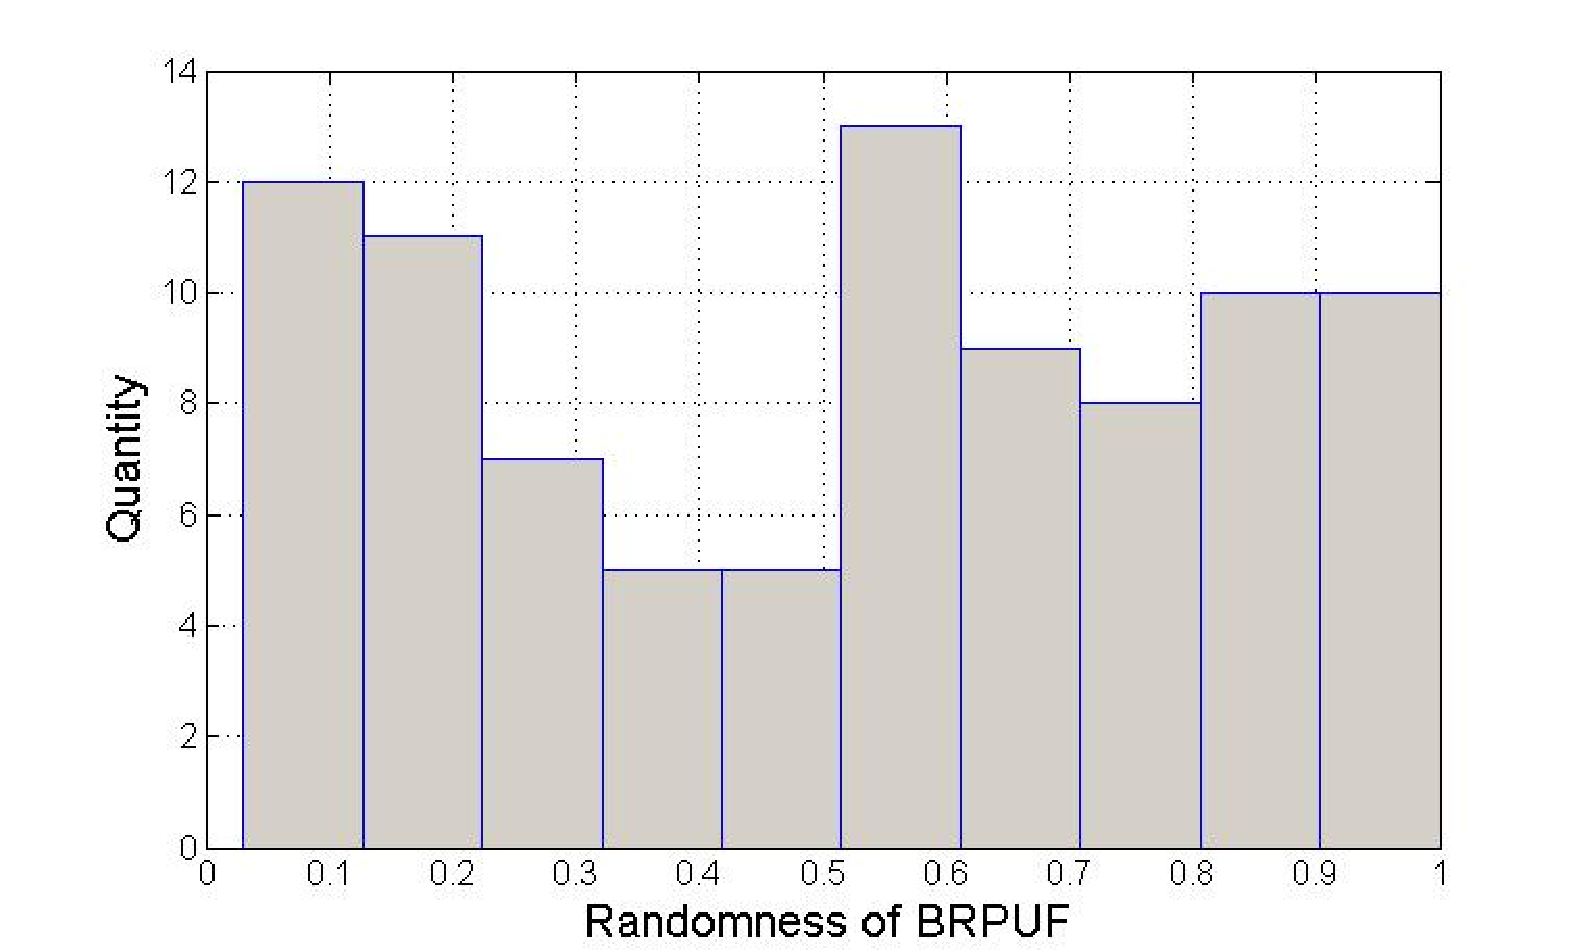
\includegraphics[width=.8\linewidth]{brpuf_rand_fpga}
}\\
\subfloat[独特性]{
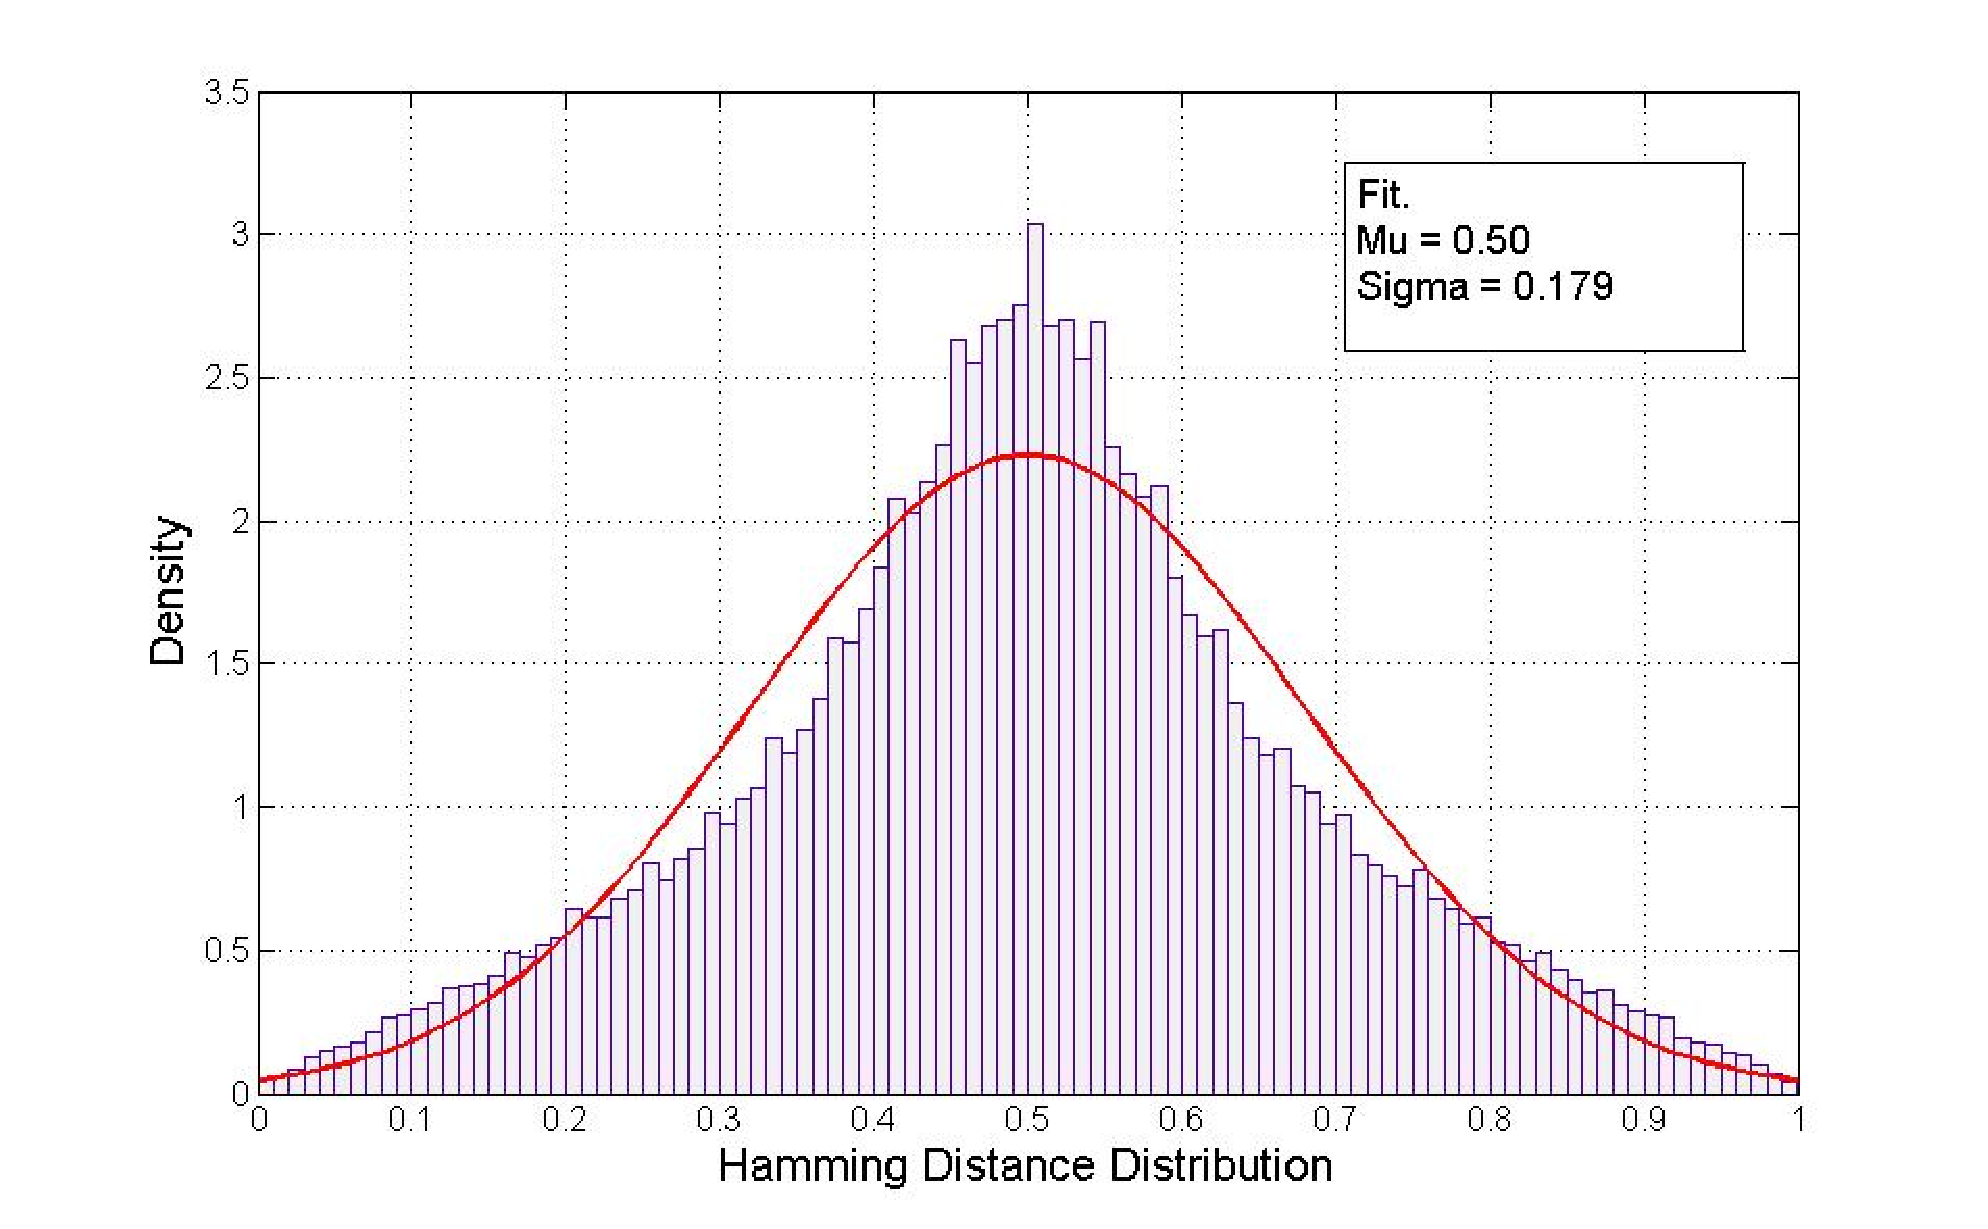
\includegraphics[width=.8\linewidth]{brpuf_uniq_fpga}
}
\caption{BRPUF FPGA实现分布}
\label{fig:brpuffpga}
\end{figure}

\begin{figure}[htb!]
\centering
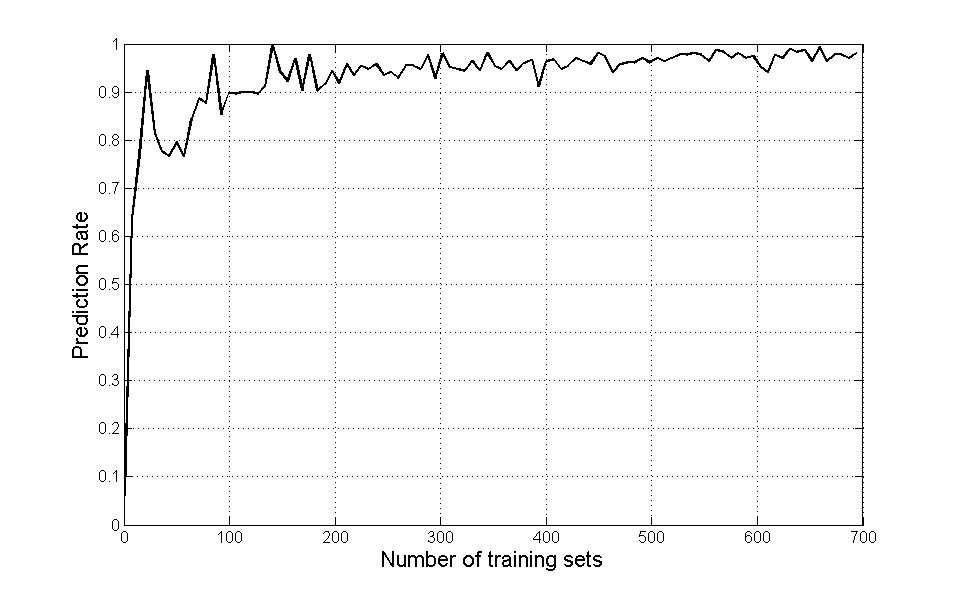
\includegraphics[width=\linewidth]{brpuf_fpga_svm.jpg}
\caption{SVM学习准确率}
\label{fig:svmfit}
\end{figure}

可以看出,预测率随训练集样本数上升的非常快,达到95\%以上的预测率仅需要200个训练样本,最终训练结果使得预测率超过99\%。

\section{本章小结}
在本章中我们首先对 BRPUF 进行了建模,根据模型分析了 BRPUF 的输出特性,由此指出其不足之处;其次提出了 PUF 在设计中遵循的原则,有利于在设计初期剔除分布较差的结构;最后通过 Matlab 和 FPGA 进行了验证并证明了我们的推论。